\section{ORS-Experiment mit einer Weißlichtquelle}\label{sec:versuchsteil2}
\subsection{Aufbau}\label{subsec:teil2_aufbau}
In diesem Versuchsteil wird die OPP-Dispersionsrelation anhand einer Silber-Luft-Grenzfläche vermessen. Dazu wird eine Weißlichtquelle (Licht
bestehend aus mehreren Wellenlängen) und ein Spektrometer verwendet. Der Versuchsaufbau dieses Versuchsteils ähnelt dem des ersten Versuchsteils und ist
in \cref{fig:versuchsteil2_aufbau} dargestellt. Die Funktion einzelner Bauteile wird nun nicht erneut erklärt (für kurze Erklärungen siehe \cref{subsec:teil1_aufbau}).
\begin{figure}[H]
	\centering
	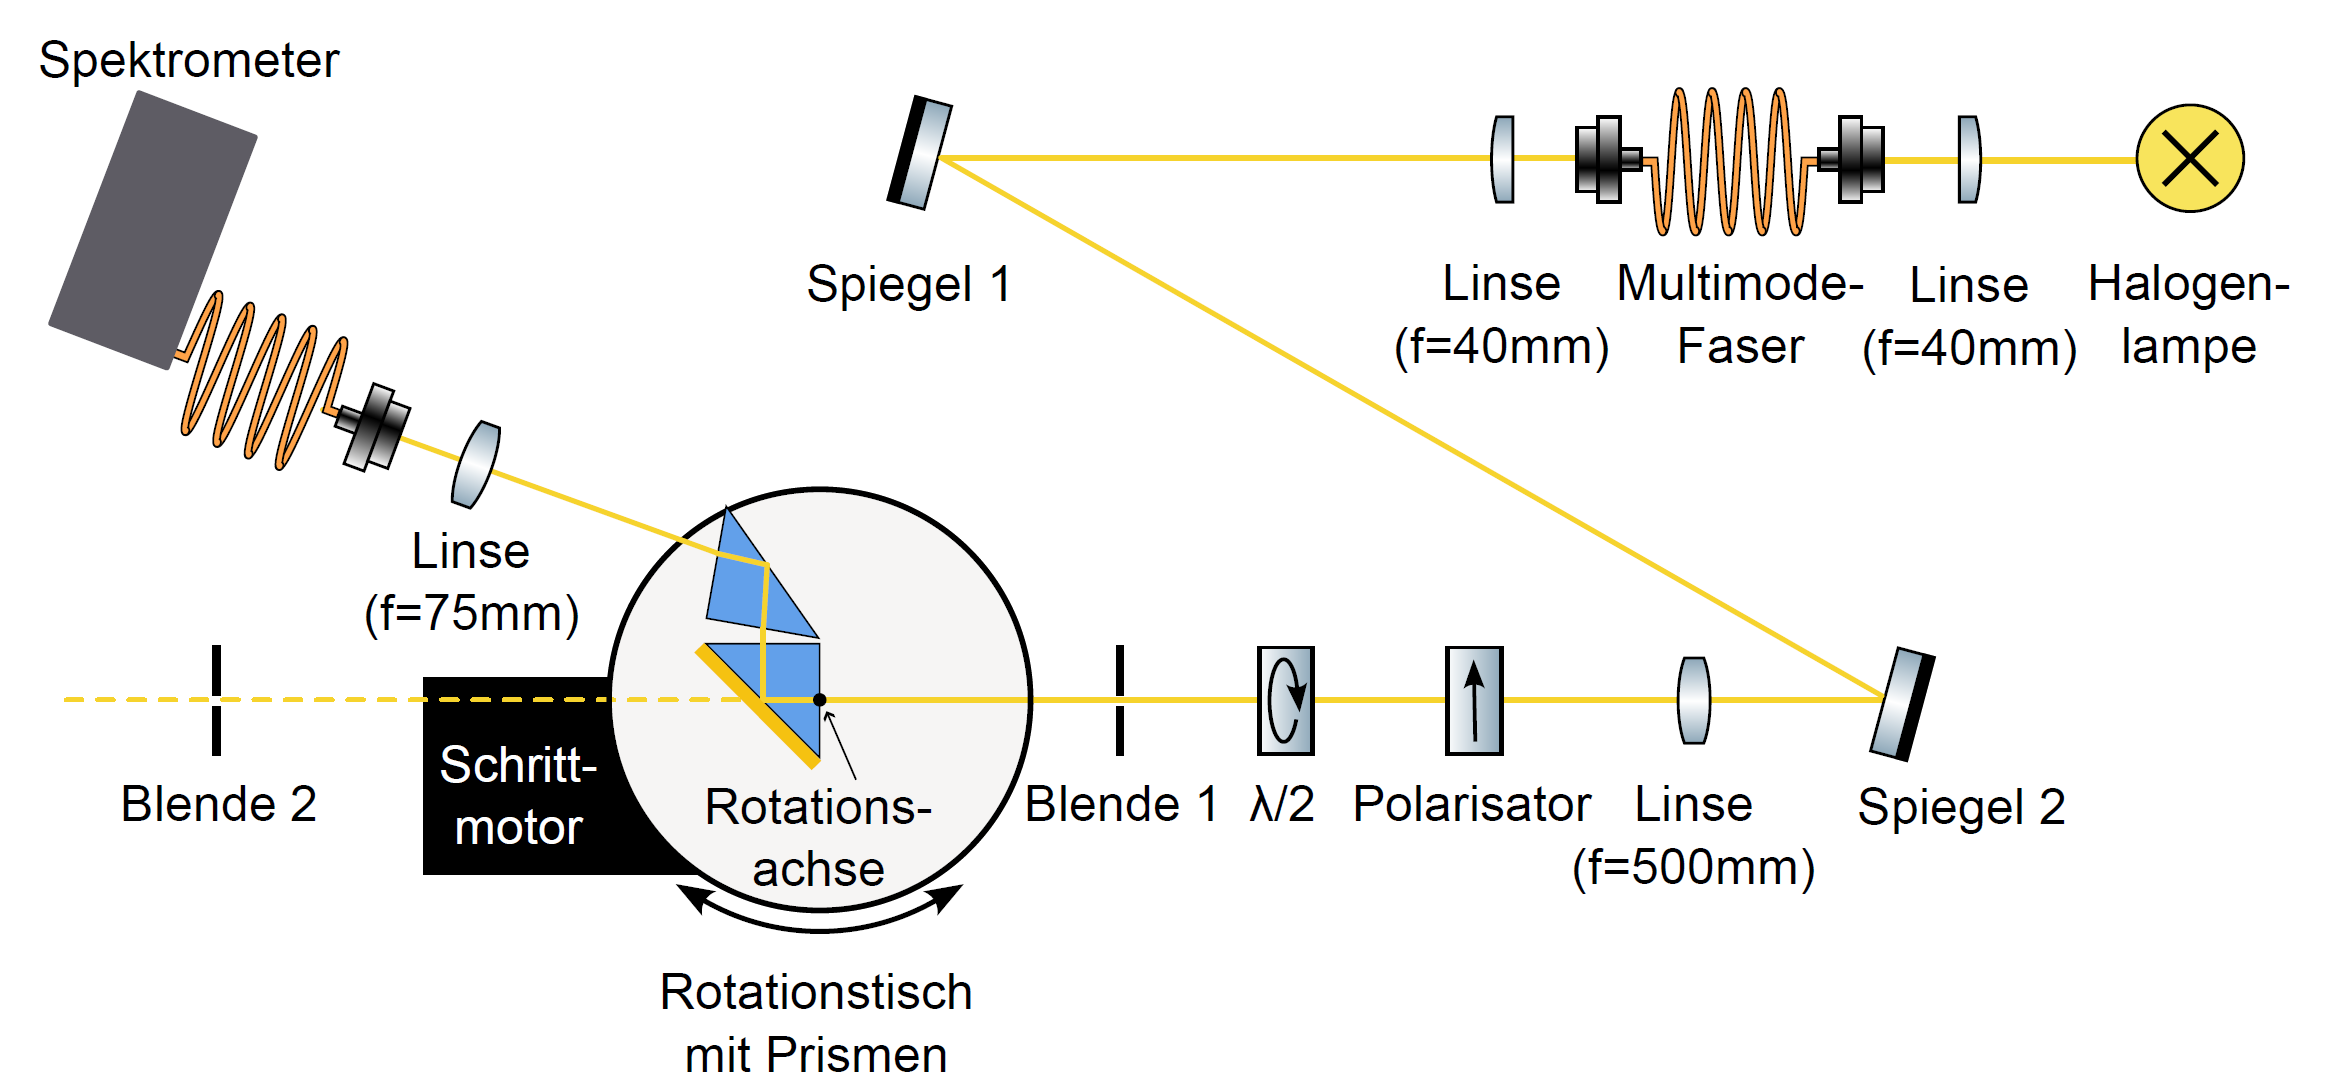
\includegraphics[width=0.6\linewidth]{../figs/versuchsteil2_aufbau.png}
	\caption{Versuchsaufbau des ORS-Experiments mit einer Weißlichtquelle und einer Zwei-Prismen-\\Konfiguration (hier ist die Linse vor der
    Multimode-Faser vor dem Spektrometer durch ein Objektiv zu ersetzen) \cite{skript}.}
	\label{fig:versuchsteil2_aufbau}
\end{figure} Als Weißlichtquelle wird eine Halogenlampe verwendet. Diese ist bereits auf dem optischen Tisch montiert. Zuerst wird das Licht der
Lampe mithilfe einer Sammellinse der Brennweite $f = \SI{40}{\mm}$ in eine Multimode-Faser gekoppelt. Diese Multimode-Faser wird verwendet, um eine
möglichst homogene Ausleuchtung zu erreichen. Vor dem Laser des ersten Versuchsteils wird dann die Ausgangsseite der Multimode-Faser platziert, wobei
die Höhe des Faserauskopplers auf etwas \SI{10}{\cm} eingestellt wird. Anschließend wird eine Sammellinse mit der Brennweite $f = \SI{40}{\mm}$ vor
den Faserauskoppler gestellt, um den Lichtstrahl zu kollimieren. Dieser Lichtstrahl muss nun analog zu dem ersten Versuchsteil justiert werden. Dafür
wird der Rotationstisch entfernt. Wieder werden die beiden Spiegel verwendet, den Lichtstrahl iterativ durch die beiden Blenden zu justieren. Hierfür
werden vorerst die Wellenplatte, der Polarisator und die Linse aus dem Strahlengang genommen und nach der Justierung des Lichtstrahls durch die beiden
Blenden wieder an die entsprechenden Positionen eingesetzt. Hierbei muss darauf geachtet werden, dass der Lichtstrahl nach dem Einsetzen der Wellenplatte,
des Polarisators und der Linse weiterhin durch beide Blenden verläuft. Nun wird auch wieder der Rotationstisch auf die vorgesehene Stelle auf dem optischen
Tisch platziert. Die Photodiode wird nun durch ein Spektrometer ersetzt, um das reflektierte Spektrum der Weißlichtquelle messen zu können.
Das reflektierte Licht wird über eine Multimode-Faser in das Spektrometer gekoppelt. Außerdem wird die Linse, die bei dem ersten Versuchsteil vor der Photodiode stand,
durch ein Objektiv ersetzt. Um die Einkopplung des Lichtstrahls in die Multimode-Faser zu optimieren, wird das Programm \texttt{ORSScan} benutzt. Da
das Spektrometer sättigt, wird die Intensität mit der Blende 1 angepasst.
\subsection{Messung}\label{subsec:teil2_messung}
Bereits vor dem Aufbau dieses Versuchsteils wurden gemeinsam mit dem Assistenten insgesamt drei Silber-Filme (jeweils mit einer Dicke von ungefähr \SI{40}{\nm}) aufgedampft. Von diesen drei Silber-Filmen wurde
nur einer für die Versuchsdurchführung benötigt. Nach dem fertiggestellten Versuchsaufbau wird der Silber-Film an der Hypotenuse des ersten Prismas befestigt.
Dann werden die Spektren des reflektierten Weißlichtstrahls mithilfe des Spektrometeres für verschiedene Einfallswinkel sowohl für TM- und TE-Polarisation gemessen.
Die SPP-Dispersionsrelation des Silber-Films wird später in der Auswertung über die SPP-Anregungswellenlängen $\lambda_{\mathrm{SPP}}$ bestimmt, welche sich
aus den winkelabhängigen lokalen Minima der Spektren bei TM-Polarisation ermitteln lassen. Für eine sinnvolle Auswertung werden daher einige dieser Minima (Anregungswellenlängen) benötigt,
weshalb bei der Messung der zu vermessende Winkelbereich so eingegrenzt wird, dass insgesamt 15 Reflexionsspektren mit jeweils (mindestens) einem lokalen Minimum aufgezeichnet werden.
Die entsprechenden Rohdaten werden erst in der Auswertung dargestellt, da sie dort direkt diskutiert werden.
\subsection{Auswertung}\label{subsec:teil2_auswertung}
Die Rohdaten für die Reflexionsspektren des Silber-Films für TM- und TE- Polarisation für den ausgewählten Winkelbereich sind in \cref{fig:silber_rohdaten} dargestellt.
Die Unsicherheit für die Wellenlänge wird zu $\Delta \lambda = \SI{0,2}{\nm}$ gewählt, was sich aus dem Abstand der Wellenlängen zweier nebeneinander liegenden Messpunkten
abschätzen lässt. Eine Unsicherheit für die reflektierte Intensität ist hier nun (im Vergleich zum ersten Versuchsteil) schwierig abzuschätzen. Prinzipiell würden
die technischen Daten der verwendeten Halogenlampe benötigt werden. Allerdings kann in guter Näherung angenommen werden, dass die Halogenlampe hinreichend stabil lief,
da sie bereits einige Zeit vor der Verwendung angeschaltet wurde, weshalb die Unsicherheiten nicht zu groß sein sollten. Darüber hinaus hängt die Unsicherheit der
gemessenen Intensität auch von dem verwendeten Spektrometer ab. Letztlich ist eine Abschätzung der Unsicherheit der Intensität aber auch überflüssig, da dies für den
quantitativen Teil der Auswertung dieses Versuchsteils nicht benötigt wird.
\begin{figure}[H]
    \centering
    \begin{subfigure}{0.45\textwidth}
        \centering
        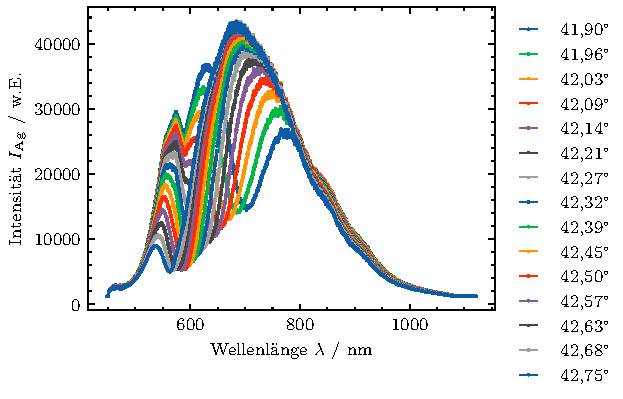
\includegraphics[width=\linewidth]{../figs/silber_tm}
        \caption{TM-Polarisation}
    \end{subfigure}
    \begin{subfigure}{0.45\textwidth}
        \centering
        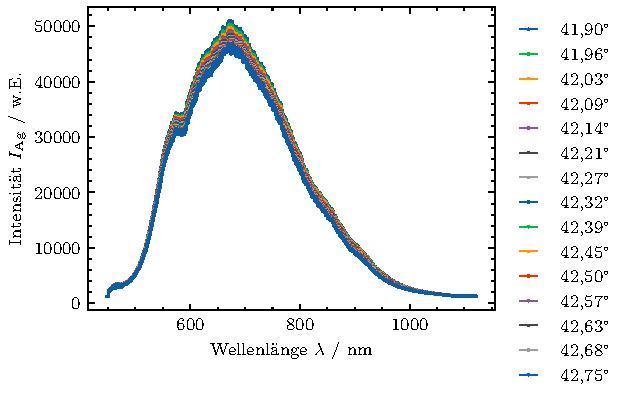
\includegraphics[width=\linewidth]{../figs/silber_te}
        \caption{TE-Polarisation}
    \end{subfigure}
    \caption{Rohdaten der Reflexionsspektren des Silber-Films für TM- und TE-Polarisation ((Wellenlängen-)Unsicherheiten sind zu klein, um erkannt zu werden).}\label{fig:silber_rohdaten}
\end{figure} In \cref{fig:silber_rohdaten} ist zunächst zu erkennen, dass wie erwartet für TE-Polarisation des einfallenden Lichtes keine OPPs angeregt werden, da sich in
den Reflexionsspektren keine lokalen Minima ausbilden. Die einfallenden Spektren werden vollständig reflektiert, weshalb die Reflexionsspektren (ungefähr) den einfallenden
Spektren entsprechenden. Das einfallende Spektrum entspricht gerade dem eines grauen Körpers, was ebenfalls der Erwartung entspricht, da eine Weißlichtquelle
verwendet wurde. Außerdem ist zu erkennen, dass die Intensitäten für unterschiedliche Winkel in etwa übereinstimmen, was für einen gut justierten Versuchsaufbau spricht.\par
Wie zu erwarten, ist in \cref{fig:silber_rohdaten} für TM-Polarisation zu erkennen, dass OPPs angeregt werden, da die Reflexionsspektren Intensitätsminima
bei den OPP-Anregungswellenlängen $\lambda_{\mathrm{OPP}}$ aufweisen. Auch hier ist wieder für jedes Reflexionsspektrum das Spektrum eines grauen Körpers zu erkennen,
wobei ein gewisser Bereich des Spektrums für die Anregung der OPPs absoriert wird. Diese Absorption geschieht nur bei einer Anregungswellenlänge $\lambda_{\mathrm{OPP}}$,
welche die Bedingungen der Energie- und Impulserhaltung erfüllt, sodass OPPs angeregt werden können.\par
Nun wird anhand der Reflexionsspektren für TM-Polarisation die OPP-Dispersionsrelation $\omega_{\mathrm{OPP}}(k_{||})$ des Silber-Films im sichtbaren Spektralbereich
bestimmt, indem für jedes Spektrum die OPP-\\Anregungswellenlänge $\lambda_{\mathrm{OPP}}$ (winkelabhängiges lokales Minimum) ermittelt wird. Dazu wird wie folgt vorgegangen:
Zunächst wird mithilfe von \cref{fig:silber_rohdaten} für das Reflexionsspektrum zu einem festen Winkel der Wellenlängenbereich, in dem die Anregungswellenlänge auftritt, grob abgelesen.
Dann wird in der entsprechenden \texttt{txt}-Datei in dem vorher eingegrenzten Wellenlängenbereich die Anregungswellenlänge rausgelesen, indem der Minimalwert
der Intensität gesucht wird. Dieses manuelle Verfahren bietet sich hier gut an, da aufgrund von minimalen Intensitätsschwankungen kein eindeutiges Minimum
festgestellt werden kann. Außerdem wird gleichzeitig eine Ableseunsicherheit abgeschätzt, je nachdem wie die Intensitätsschwankungen ausfallen, was dann z.B.
zu einem etwas größeren oder kleineren Wellenlängenbereich für die tatsächliche Anregungswellenlänge führt.\par
Nach \cite{skript} wird dann der zugehörige Wellenvektor gemäß
\begin{equation*}
	k_{||} = \frac{2\pi n_{\mathrm{Prisma}}}{\lambda_{\mathrm{OPP}}} \sin(\theta)
\end{equation*} berechnet, wobei die Unsicherheit durch
\begin{equation*}
	\Delta k_{||} = \sqrt{\left(\frac{2\pi n_{\mathrm{Prisma}}}{\lambda_{\mathrm{OPP}}^2} \sin(\theta) \Delta \lambda_{\mathrm{OPP}}\right)^2 + \left(\frac{2\pi n_{\mathrm{Prisma}}}{\lambda_{\mathrm{OPP}}} \cos(\theta) \Delta \theta\right)^2}
\end{equation*} gegeben ist. Die Unsicherheit $\Delta \theta = \SI{0,06}{\degree}$ wird hier wieder aus der Anzahl an Winkelmessungen in dem gewählten Winkelbereich abgeschätzt.
Die Anregungskreisfrequenz berechnet sich durch
\begin{equation*}
	\omega_{\mathrm{OPP}} = \frac{2\pi c_0}{\lambda_{\mathrm{OPP}}}
\end{equation*} mit der Unsicherheit
\begin{equation*}
	\Delta \omega_{\mathrm{OPP}} = \frac{2 \pi c_0}{\lambda_{\mathrm{OPP}}^2} \Delta \lambda_{\mathrm{OPP}} .
\end{equation*} Die Werte für $\lambda_{\mathrm{OPP}}$ und die daraus berechneten Werte für $k_{||}$ und $\omega_{\mathrm{OPP}}$ sind in \cref{tab:dispersionsrelation}
dargestellt.
\begin{table}[H]
    \centering
    \caption{Anregungswellenlängen $\lambda_{\mathrm{OPP}}$ und die zugehörigen Wellenvektoren $k_{||}$ bzw. die zugehörigen Anregungskreisfrequenzen
	$\omega_{\mathrm{OPP}}$ des Silber-Films für einen bestimmten ausgewählten Winkelbereich.}
    \begin{tabular}{c|c|c}
        $\lambda_{\mathrm{OPP}}$ / \unit{\nm} & $k_{||}$ / \unit{\per\nm} & $\omega_{\mathrm{OPP}} \cdot 10^{15}$ / \unit{\per\second} \\
        \hline
        \num{562(2)} & $\num{0,01138(5)}$ & $\num{3,352(12)}$ \\
        \num{568(2)} & $\num{0,01125(5)}$ & $\num{3,316(12)}$ \\
        \num{577(2)} & $\num{0,01106(5)}$ & $\num{3,265(12)}$ \\
        \num{584(2)} & $\num{0,01092(4)}$ & $\num{3,225(12)}$ \\
		\num{590(2)} & $\num{0,01079(4)}$ & $\num{3,193(11)}$ \\
		\num{596(2)} & $\num{0,01067(4)}$ & $\num{3,160(11)}$ \\
		\num{604(2)} & $\num{0,01052(4)}$ & $\num{3,119(11)}$ \\
		\num{613(2)} & $\num{0,01035(4)}$ & $\num{3,073(10)}$ \\
		\num{623(2)} & $\num{0,01018(4)}$ & $\num{3,024(10)}$ \\
		\num{634(2)} & $\num{0,00999(4)}$ & $\num{2,971(10)}$ \\
		\num{644(2)} & $\num{0,00982(4)}$ & $\num{2,925(10)}$ \\
		\num{654(3)} & $\num{0,00966(5)}$ & $\num{2,880(14)}$ \\
		\num{669(3)} & $\num{0,00943(5)}$ & $\num{2,816(13)}$ \\
		\num{685(4)} & $\num{0,00920(6)}$ & $\num{2,740(17)}$ \\
		\num{703(4)} & $\num{0,00895(6)}$ & $\num{2,679(16)}$                 
    \end{tabular}\label{tab:dispersionsrelation}
\end{table} Diese Werte sind nun als OPP-Dispersionsrelation $\omega_{\mathrm{OPP}}(k_{||})$ in \cref{fig:darstellung_dispersionsrelation} zusammen mit
der Lichtlinie $\omega_{\mathrm{Licht}}(k_{||}) = c_0 k_{||}$ aufgetragen.
\begin{figure}[H]
	\centering
	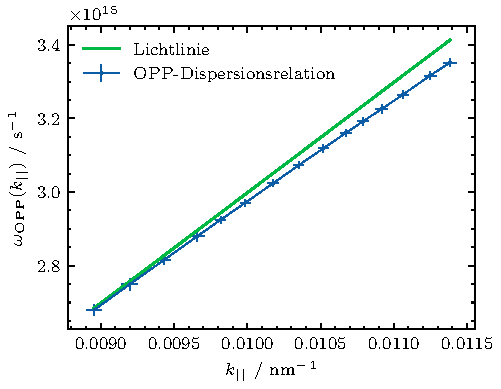
\includegraphics[width=0.6\linewidth]{../figs/dispersionsrelation_opp.pdf}
	\caption{Vergleich der OPP-Dispersionsrelation von Silber mit der Dispersionsrelation von Licht.}
	\label{fig:darstellung_dispersionsrelation}
\end{figure} Hier entsprechen die Ergebnisse den theoretischen Erwartungen, wenn ein Vergleich mit \cref{fig:dispersion} herangezogen wird. Gemäß der
theoretischen Erwartung laufen in \cref{fig:darstellung_dispersionsrelation} die OPP-Dispersionsrelation für Silber und die Lichtlinie für kleiner
werdende $k_{||}$ asymptotisch gegeneinander. Für größer werdende $k_{||}$ laufen jedoch die OPP-Dispersionsrelation für Silber und die Lichtlinie
zunehmend auseinander, was ebenfalls der theoretischen Erwartung entspricht. Um allgemeingültige Aussagen treffen zu können, hätte ein noch größerer
Wellenlängenbereich betrachtet werden müssen. Da die hier dargestellte OPP-Dispersionsrelation $\omega_{\mathrm{OPP}}(k_{||})$ nur für den
sichtbaren Spektralbereich (siehe die ermittelten Anregungswellenlängen) bestimmt wurde, ist diese Diskussion dieser auch nur für den sichtbaren Spektralbereich gültig.
Im sichtbaren Spektralbereich (nach den theoretischen Erwartungen sogar über einen wesentlich breiteren Spektralbereich) kommt es gemäß \cref{fig:darstellung_dispersionsrelation}
tatsächlich zu keinem Schnittpunkt der OPP-Dispersionsrelation für Silber und der Lichtlinie, womit im Rahmen der Unsicherheiten bestätigt ist, dass im sichtbaren Spektralbereich
für Licht, welches aus Luft kommend auf die Dielektrikum-Silber-Grenzfläche (Luft-Silber-Grenzfläche) trifft, keine OPPs angeregt werden können, da tatsächlich die
Bedingung $k_{\mathrm{OPP},||} = \frac{\omega}{c_0}$ nicht erfüllt ist. Somit zeigt sich auch, dass die Kretschmann-Konfiguration während der Versuchsdurchführung
unabdingbar war, um OPPs anregen zu können.